\graphicspath{{Kapitel/Kapitel4_Hauptteil/Images/}}

Dieses Kapitel beschreibt die Virtual Reality Applikation \textbf{C.LABEL-VR} und ist somit der Hauptteil dieser Arbeit. Das Ziel dieser Applikation ist es die Annotierung von Punktwolken, wie sie beispielsweise in \textbf{C.LABEL}(siehe Kapitel \ref{sec:C.LABEL}) möglich ist, innerhalb einer dreidimensionalen Umgebung zu realisieren. Dazu müssen Datenformate, welche Informationen über Punktwolken enthalten, eingelesen und anschließend, aus diesen Daten, Punktwolken generiert werden. Der Vorgang des Imports wird in Kapitel \ref{sec:ImportExport} näher beschrieben, die Generierung der Punktwolken in \ref{sec:Generierung}. Um sich in der virtuellen Umgebung durch diese Wolken zu bewegen, wurden diverse Möglichkeiten zur Navigation entwickelt. Auf die Funktion dieser Möglichkeiten und deren Auswirkungen auf das befinden des Menschen (\textit{Virtual Motion Sickness}) wird in Kapitel \ref{sec:Navigation} eingegangen. Anschließend geht es um die Annotierung der generierten Punktwolken. Annotierung bedeutet in diesem Kontext, dass die einzelnen Punkte der Wolken mit bestimmten Klassifikationen versehen werden, welche der Art des Objektes entsprechen, dem der Punkt zugehört. Ist der Punkt beispielsweise Bestandteil eines Autos, so wird er mit der Klasse \glqq Auto\grqq versehen. Um diese Aufgabe erfüllen zu können gibt wurden mehrere Arten der Annotierung entwickelt. Welche dies sind und wie sie realisiert wurden, ist in Kapitel \ref{sec:Annotation} erklärt. Das letzte Kapitel \ref{sec:UIMenu} beschäftigt sich mit dem User Interface der Applikation. Dabei wird hauptsächlich auf die Funktionen des Ingame-Menüs eingegangen, welche Herausforderungen es bei der Erstellung von \acrshort{acr:UI}s in der virtuellen Realität gibt und wie diese bewältigt wurden. Zur Veranschaulichung der Funktionen von \textbf{C.LABEL-VR} ist in der Abbildung \ref{fig:Workflow} der grobe \gls{glos:Workflow} in Form eines Diagramms abgebildet.

\begin{figure}%
	\centering
    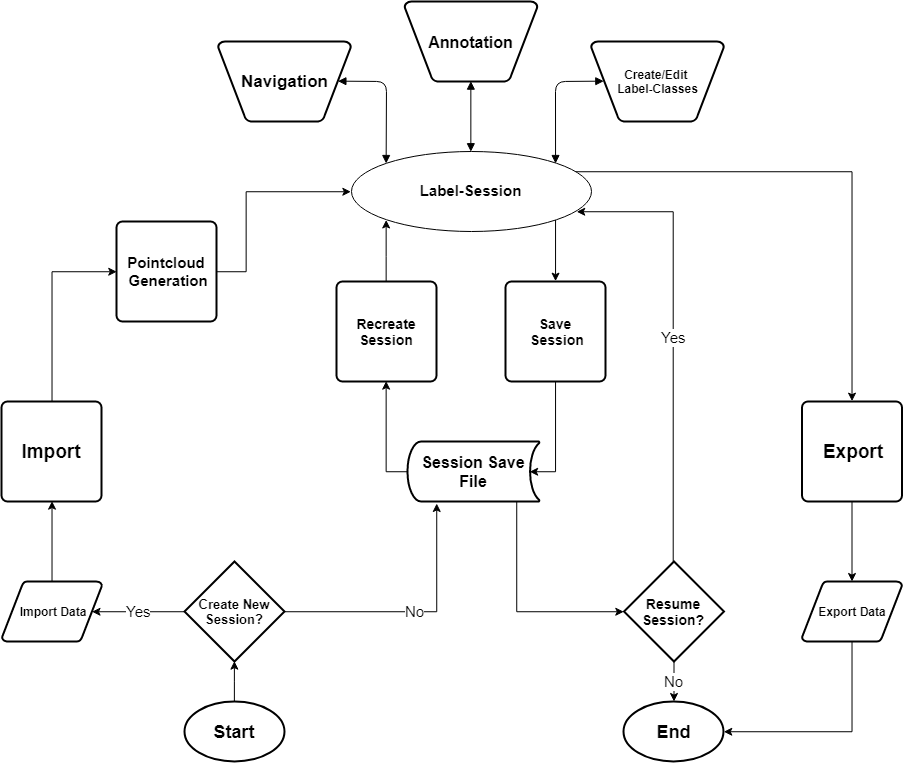
\includegraphics[width=13.5cm]{Workflow}
    \caption{\glslink{glos:Workflow} in C.LABEL-VR vom Import bis zum Export}
    \label{fig:Workflow}
\end{figure}

\section{Import und Export von Daten}
\label{sec:ImportExport}
Umfeldmodelle, welche in Form einer Punktwolke vorliegen, werden meist von einem Radar-, oder wie in Kapitel \ref{sec:Lidar} von einem Lidar-Sesnor aufgenommen. Die Informationen über diese Modelle, zum Beispiel die Positionen der einzelnen Punkte, werden in einem passenden Datenformat abgespeichert. Um welches Format es sich dabei handelt kann sehr unterschiedlich sein. In der Regel hängt es davon ab zu welchem Zweck die aufgenommenen Daten gebraucht werden und wie umfangreich diese Daten sind. Am häufigsten werden sie dafür verwendet um Lernalgorithmen und neuronale Netze (siehe \ref{sec:KNN}) zu trainieren. Automobilhersteller beispielsweise haben für solche vorhaben natürlich unterschiedliche Konzepte und somit können auch die Formate der Daten unterschiedlich sein.\\ 

Innerhalb dieser Arbeit wurden mit zwei verschiedenen Arten von Daten gearbeitet. Die \gls{glos:OpenSrc}-Bibliothek \textbf{PCL}(\textit{Point Cloud Library}) benutzt das Datenformat \textbf{PCD}(\textit{Point Cloud Data}) um Informationen über Punktwolken einzulesen. PCL ist eine sehr mächtige C++-Bibliothek, die in der Regel von jedem benutzt wird, der performante Algorithmen für Punktwolken entwickeln möchte. Auch C.LABEL (siehe \ref{sec:C.LABEL}) generiert aus eingelesenen Daten PCD-Files um Funktionen der Point CLoud Library für die Wolken zu benutzen.

Das zweite Format ist das, von der HDF-Group bereitgestellte \textbf{HDF5}(\textit{Heterogeneous Data Format}). Es ist ausgelegt zur schnellen Erstellung und Auslesung von komplexen Datenstrukturen. Wie diese Strukturen aussehen wird später in Kapitel \ref{sec:HDF5} näher erklärt. Zur schnellen Bearbeitung großer Datenmengen ist dies ein gängiges Format, wird von den meisten Kunden von CMORE benutzt und deshalb auch in C.LABEL-VR verwendet.\\

\subsection{Architektur}

Wichtig ist es also sowohl den Import, als auch den Export so modular wie möglich zu gestalten, dass er leicht um neue Datenformate erweitert werden kann. Diese Erweiterungen werden im Folgenden \textbf{Addons} genannt. Aber nicht nur unterschiedliche Arten von Daten, auch Komplexe Formate wie HDF5, welche anpassbare Strukturen haben, müssen für jede Struktur, auf unterschiedliche Weise eingelesen werden und brauchen somit auch separate \glqq Importer-\grqq und \glqq Exporter\grqq -Addons. Um dies zu bewerkstelligen wurde eine interne Datenstruktur(\acrshort{acr:IDS}) eingeführt, die alle nötigen Informationen enthält, die für das \gls{glos:Labeling} notwendig sind. Diese wird im späteren Kapitel \ref{sec:IDS} vorgestellt. Der Vorteil dabei ist, dass man dadurch nach dem Import bis zum Export auf die gleiche Datenstruktur zurückgreifen kann und somit unabhängig vom importierten Datenformat ist. Wird also ein neues Import-Format eingeführt muss an der Hauptapplikation nichts verändert werden. \\ 

Jedes Import-Addon hat also zunächst die Aufgabe, seine jeweiligen Daten einzulesen und alle Informationen, die für die \acrshort{acr:IDS} notwendig sind, daraus zu extrahieren. Aus diesen Informationen können anschließend die entsprechenden Punktwolken generiert werden (siehe \ref{sec:PclGenerate}). Beim Export ist es notwendig, dass die Struktur der, vom Addon eingelesenen Daten, gleich bleibt. Es sollen lediglich die \gls{}glos:Labeling}-Informationen aus der \acrshort{acr:IDS} hinzu- bzw. eingefügt werden. Die Importierten Daten, beispielsweise \textbf{HDF5}, enthalten allerdings oft deutlich mehr Informationen, als für die interne Struktur notwendig. Diese Zusatzinformationen werden \textbf{Metadaten} genannt. Für den Export bedeutet dies, dass man aus der internen Struktur von \textbf{C.LABEL-VR} die Struktur, der anfangs eingelesenen Daten, nicht wieder rekonstruieren kann. \\

   METADATEN

\begin{figure}%
	\centering
    \includegraphics[width=13.5cm]{Import_Export_Architecture}
    \caption{Das Import-Export-Prinzip in C.LABEL-VR}
    \label{fig:Workflow}
\end{figure}

\subsection{HDF5-Beispiel}
\subsubsection{HDF5 Daten}
\label{sec:HDF5}
\subsubsection{Beispiel}

\section{Generierung einer Punktwolke}
\label{sec:Generierung}

\subsection{Interne Datenstruktur}
\label{sec:IDS}

\subsection{Generierung}
\label{sec:PclGenerate}
session
pointcloud
...

Koordinatensysteme

\subsection{Optimierung}
-generell nichts teures in update mehthode
	
-gameobject find
-getcomponent

keine update oder start mehtode bei skripten der punkte
collider trigger nicht bei den punkten sondern beim anderen object
generell alle pollenden aktionen von den punkten entfernen


(-clonen von prefabs statt neue instanzen von inbuilts)
shared materials verwenden   kein material.color weil das eine kopie des materials erzeugt, welches dann einzeln gecallt werden muss

gpu instancing bei den materials verwenden und forward rendering options

\section{Navigation}
\label{sec:Navigation}
\subsection{VR-Krankheit}
\subsection{Freier Flug}
\subsection{Teleport}

\section{Annotieren der Punktwolke}
\label{sec:Annotation}
\subsection{Pointer Labeling}
\subsection{Clustering}
\subsubsection{ground plane fitting}
%https://en.wikipedia.org/wiki/Singular-value_decomposition
%https://www.ltu.se/cms_fs/1.51590!/svd-fitting.pdf

\section{Ingame Menu}
\label{sec:UIMenu}
\subsection{Movement}
\subsection{Labelclasses}


